\onehalfspacing
We illustrate application of the GA on an example containing 20 synthetic fault-slip observations shown in Fig. 6.A. For brevity, we consider an initial population size of 20 tensors over a single iteration. The actual implementation typically uses a population size of 1000 for 100 iterations.

\section{Initialization and Encoding}
The reduced stress tensor depends on four parameters $\alpha, \beta, \gamma$ and $\phi$ that are estimated using the stress inversion. The ranges of these parameters are defined in Section 2.3, Chapter 2. In order to encode the parameters in binary, we divide them into $2^n$ equal parts, $n$ being a positive integer. Here, we choose $n = 6$ for each parameter, so that each parameter is divided into 64 equal parts, numbered 0 to 63. Any choice of larger values gives better precision at cost of computation time.

We assign random integers, ranging from 0 to 63, to the parameters $\alpha, \beta, \gamma$ and $\phi$ (Table 4). These integers are then converted into 6-bit binary strings for each parameter, i.e., 24 bits in total, for the subsequent operations of the GA. We will generate a set of 20 non negative integers for each parameter, which is the initial population.

Next, we encode the parameters in real space as follows:
\begin{align} \label{222}
\begin{split}
    \alpha_{real} &= (2\pi) \times (1/63) \times \alpha, \\
    \beta_{real} &= (\pi/2) \times (1/63) \times \beta, \\
    \gamma_{real} &= (2\pi) \times (1/63) \times \gamma, \\
    \phi_{real} &= (1/63) \times \phi.
\end{split}
\end{align}

Thus, the integer values of$\alpha, \beta$ and $\gamma$ are converted into radians and that of $\phi$ into a ratio. For example, if the first value of $\alpha$ is 26, then its real value is $26 \times 2\pi \times (1/63) = 2.59$ and its six bit binary representation is 011010 (Table 4). One set of binary values of $\alpha, \beta, \gamma$ and $\phi$ defines an individual. $\alpha_{real}, \beta_{real}, \gamma_{real}$ and $\phi_{real}$ are substituted in Eqs. 3 and 4 in the main text to get the reduced stress tensor.

\section{Misfit Calculation}
Each fault is characterized by a normal vector and a slip vector (Eqs. 1 and 2). These vectors are used to calculate the fitness of an individual using the misfit function (Eq. 17). For each one of the 20 initial stress tensors, the mean misfit is calculated (Table 4). The stress tensor having a lower misfit is a better solution to the inverse problem and will be preferred than the one having higher misfit.

\section{Tournament Selection}
Next, 20 pairs of individuals are randomly chosen for competing against each other (Table 4). From each pair, the individual with a lower misfit is declared as the winner, who is represented by four parameters, $m_{\alpha}, m_{\beta}, m_{\gamma}$ and $m_{\phi}$ (Table 4). Table 5 shows the mating pool of winners in binary format.

\pagebreak

\begin{table}[htb]
  \footnotesize
  \centering
   \renewcommand{\arraystretch}{1.2}
  \begin{tabular}{@{}lccccc|cccccc@{}}
    \toprule
    S.No. & $\alpha$ & $\beta$ & $\gamma$ & $\phi$ & Misfit & Tournament & Winner & $m_{\alpha}$ & $m_{\beta}$ & $m_{\gamma}$ & $m_{\phi}$ \\
    \midrule
    1 & 26 & 45 & 52 & 8 & 0.3376 & 9 \& 18 & 9 & 39 & 14 & 0 & 18 \\
    2 & 63 & 20	& 2	& 10 & 0.1415 & 11 \& 16 & 16 & 16 & 26 & 50 & 26 \\
    3 & 57 & 59 & 12 & 13 & 0.3328 & 6 \& 18 & 6 & 52 & 39 & 1 & 53 \\
    4 & 33 & 25	& 32 & 29 & 0.2272 & 11 \& 12 & 11 & 23 & 33 & 24 & 15 \\
    5 & 61 & 14	& 16 & 59 & 0.3222 & 7 \& 12 & 7 & 42 & 15 & 31 & 54 \\ 
    6 & 52 & 39	& 1 & 53 & 0.2378 & 20 \& 12 & 20 & 53 & 49 & 18 & 50 \\
    7 & 42 & 15 & 31 & 54 & 0.2290 & 16 \& 3 & 16 & 16 & 26 & 50 & 26 \\
    8 & 24 & 36 & 26 & 8 & 0.2725 & 15 \& 7 & 15 & 1 & 8 & 57 & 59 \\
    9 & 39 & 14 & 0 & 18 & 0.0795 & 18 \& 11 & 11 & 23 & 33 & 24 & 15 \\
    10 & 4 & 28 & 61 & 61 & 0.2580 & 18 \& 5 & 5 & 61 & 14 & 16 & 59 \\
    11 & 23	& 33 & 24 & 15 & 0.2493 & 19 \& 8 & 8 & 24 & 36 & 26 & 8 \\
    12 & 15	& 52 & 16 & 18 & 0.3475 & 17 \& 10 & 17 & 52 & 6 & 21 & 18 \\
    13 & 22	& 35 & 30 & 2 & 0.2503 & 14 \& 14 & 14 & 36 & 27 & 2 & 46 \\
    14 & 36	& 27 & 2 & 46 & 0.2507 & 9 \& 6	& 9 & 39 & 14 & 0 & 18 \\
    15 & 1 & 8 & 57 & 59 & 0.1742 & 6 \& 20	& 6 & 52 & 39 & 1 & 53 \\ 
    16 & 16	& 26 & 50 & 26 & 0.1667 & 15 \& 13 & 15 & 1 & 8 & 57 & 59 \\
    17 & 52	& 6 & 21 & 18 & 0.0829 & 6 \& 6 & 6 & 52 & 39 & 1 & 53 \\
    18 & 27	& 54 & 17 & 12 & 0.3507 & 11 \& 8 & 11 & 23 & 33 & 24 & 15 \\
    19 & 22	& 44 & 29 & 16 & 0.3156 & 12 \& 5 & 5 & 61 & 14 & 16 & 59 \\
    20 & 53	& 49 & 18 & 50 & 0.2593 & 2 \& 7 & 2 & 63 & 20 & 2 & 10 \\
    \cmidrule(lr){5-6}
     & & & & Avg.= & 0.2443 & & & & & & \\

    \bottomrule
  \end{tabular}
  \caption{Initialization, encoding and tournament selection. The `Tournament` column represents the serial number of the stress tensor parameters chosen for competing. The `Winner` column also represents the serial number, and corresponds to the one with lower misfit. Last four columns are the winners, i.e., the mating pool.}\label{table:4}
\end{table}

\section{Crossover and Mutation}
The threshold\% for crossover is subjective. On the basis of numerous trials on various synthetic sets, we found that a threshold 80\% gives satisfactory and time efficient results. Following this, we randomly selected 80\% of the 20 individuals in the mating pool for crossover. The remaining 20\% go to the next stage without any crossover.

Next, two random individuals are selected, and two random crossover sites are chosen. Using the process of two-point crossover, the offspring are generated by exchanging the bits in between the crossover sites (Fig. 4A-B, Table 5). In the next stage, to implement mutation, one random bit of any one offspring, chosen with a very low probability, usually 1/number of bits, is flipped from 1 to 0, or 0 to 1. The mutation slows down the convergence of the algorithm so that it does not get entrapped in a local optimum. The 24 bit offspring is then divided into four equal parts, each 6-bit long, representing the parameters $m_{\alpha}, m_{\beta}, m_{\gamma}$ and $m_{\phi}$ of the newly created stress-tensor (Table 6). Now these parameters are treated as the next generation and the entire process of selection, crossover and mutation is repeated until a good solution is obtained.

\begin{table}[htb]
  \footnotesize
  \centering
  %\setlength{\tabcolsep}{5pt}
  \renewcommand{\arraystretch}{1.2}
  \begin{tabular}{@{} l c p{1.5cm} p{1.5cm} c @{}}
    \toprule
    S.No. & Mating Pool & Crossover between & Crossover sites & Offspring \\
   \midrule    
    1 & 100111001110000000010010 & 19 \& 18 & 8 \& 15 &  111101000001011000111011 \\
    
    2 & 010000011010110010011010 & -- & -- & 010111101110010000001111 \\
    
    3 & 110100100111000001110101 & 8 \& 5 & 7 \& 14 & 000001001111011001111011 \\

    4 & 010111100001011000001111 & -- & -- & 101010001000111111110110 \\

    5 & 101010001111011111110110 & 9 \& 3 & 6 \& 17 & 	010111100111000000001111 \\
    
    6 & 110101110001010010110010 & -- & -- & 110100100001011001110101 \\
    
    7 & 010000011010110010011010 & 8 \& 7 & 10 \& 12 & 000001001010111001111011 \\
    
    8 & 000001001000111001111011 & -- & -- & 010000011000110010011010 \\

    9 & 010111100001011000001111 & 5 \& 17 & 5 \& 10 & 	101010100111011111110110 \\

    10 & 111101001110010000111011 & -- & -- & 110100001111000001110101 \\

    11 & 011000100100011010001000 & 8 \& 16 & 12 \& 18 & 	000001001000111001111011 \\
    
    12 & 110100000110010101010010 & -- & -- & 000001001000111001111011 \\
    
    13 & 100100011011000010101110 & 20 \& 20 & 3 \& 13 & 	111111010100000010001010 \\
    
    14 & 100111001110000000010010 & -- & -- & 111111010100000010001010 \\
    
    15 & 110100100111000001110101 & 19 \& 18 & 1 \& 13 & 	110111100001010000111011 \\
    
    16 & 000001001000111001111011 & -- & -- & 011101001110011000001111 \\
    
    17 & 110100100111000001110101 & --- & --- & 110100100111000001110101 \\
    
    18 & 010111100001011000001111 & --- & --- & 010111100001011000001111 \\
    
    19 & 111101001110010000111011 & --- & --- & 111101001110010000111011 \\
    
    20 & 111111010100000010001010 & --- & --- & 111111010100000010001010 \\

    \bottomrule
  \end{tabular}
  \caption{Crossover. The third column shows the individuals randomly selected for crossover. Crossover sites are the position between which the bits are exchanged. 20\% of the members that go to next generation without any crossover are shown in S.No. 17 to 20.}\label{table:5}
\end{table}

\pagebreak

\begin{table}[htb]
  \footnotesize
  \centering
  %\setlength{\tabcolsep}{5pt}
  \renewcommand{\arraystretch}{1.2}
  \begin{tabular}{@{}c c c c c@{}}
    \toprule
    $ Offspring_{\alpha}$ & $ Offspring_{\beta}$ & $ Offspring_{\gamma}$ & $ Offspring_{\phi}$ & Misfit \\
   \midrule    
   
    61 & 1 & 24 & 59 & 0.1992 \\
    1 & 15 & 25 & 59 & 0.1972 \\
    23 & 39 & 0 & 15 & 0.2881 \\
    1 & 10 & 57 & 59 & 0.1898 \\
    42 & 39 & 31 & 54 & 0.2692 \\
    1 & 8 & 57 & 59 & 0.1742 \\
    63 & 20 & 2 & 10 & 0.1415 \\
    55 & 33 & 16 & 59 & 0.2497 \\
    29 & 14 & 16 & 15 & 0.1077 \\
    63 & 20 & 2 & 10 & 0.1415 \\
    1 & 8 & 57 & 59 & 0.1742 \\
    52 & 15 & 31 & 53 & 0.2237 \\
    16 & 24 & 57 & 26 & 0.1982 \\
    52 & 33 & 0 & 53 & 0.2288 \\
    42 & 8 & 25 & 54 & 0.1657 \\
    23 & 46	& 24 & 15 & 0.3158 \\
    39 & 14	& 0 & 18 & 0.0795 \\
    52 & 39	& 1 & 53 & 0.2387 \\
    61 & 14	& 16 & 59 & 0.3222 \\
    52 & 39	& 1 & 53 & 0.2387 \\
    \cmidrule(lr){4-5}
     & & & Avg. = & 0.2072 \\
   
    \bottomrule
  \end{tabular}
  \caption{Decoding the offspring for the next iteration. The last column shows the misfit. Last row shows average that is compared with average in Table 4.}\label{table:6}
\end{table}

The average misfit of the population is reduced from 0.2443 in the parents to 0.2072 in the offspring (compare Tables 4 and 6). Thus, the second generation population consists of better fit individuals than the first generation. If we were to stop here, the parameters corresponding to the lowest misfit from this pool of the individuals would define the desired reduced stress tensor. Ideally, for a large number of iterations, the final population will converge towards the same value for every member of the population, which will represent the optimum stress tensor.
\pagebreak

\begin{figure}[h!]
\begin{subfigure}{\textwidth}
    \centering
    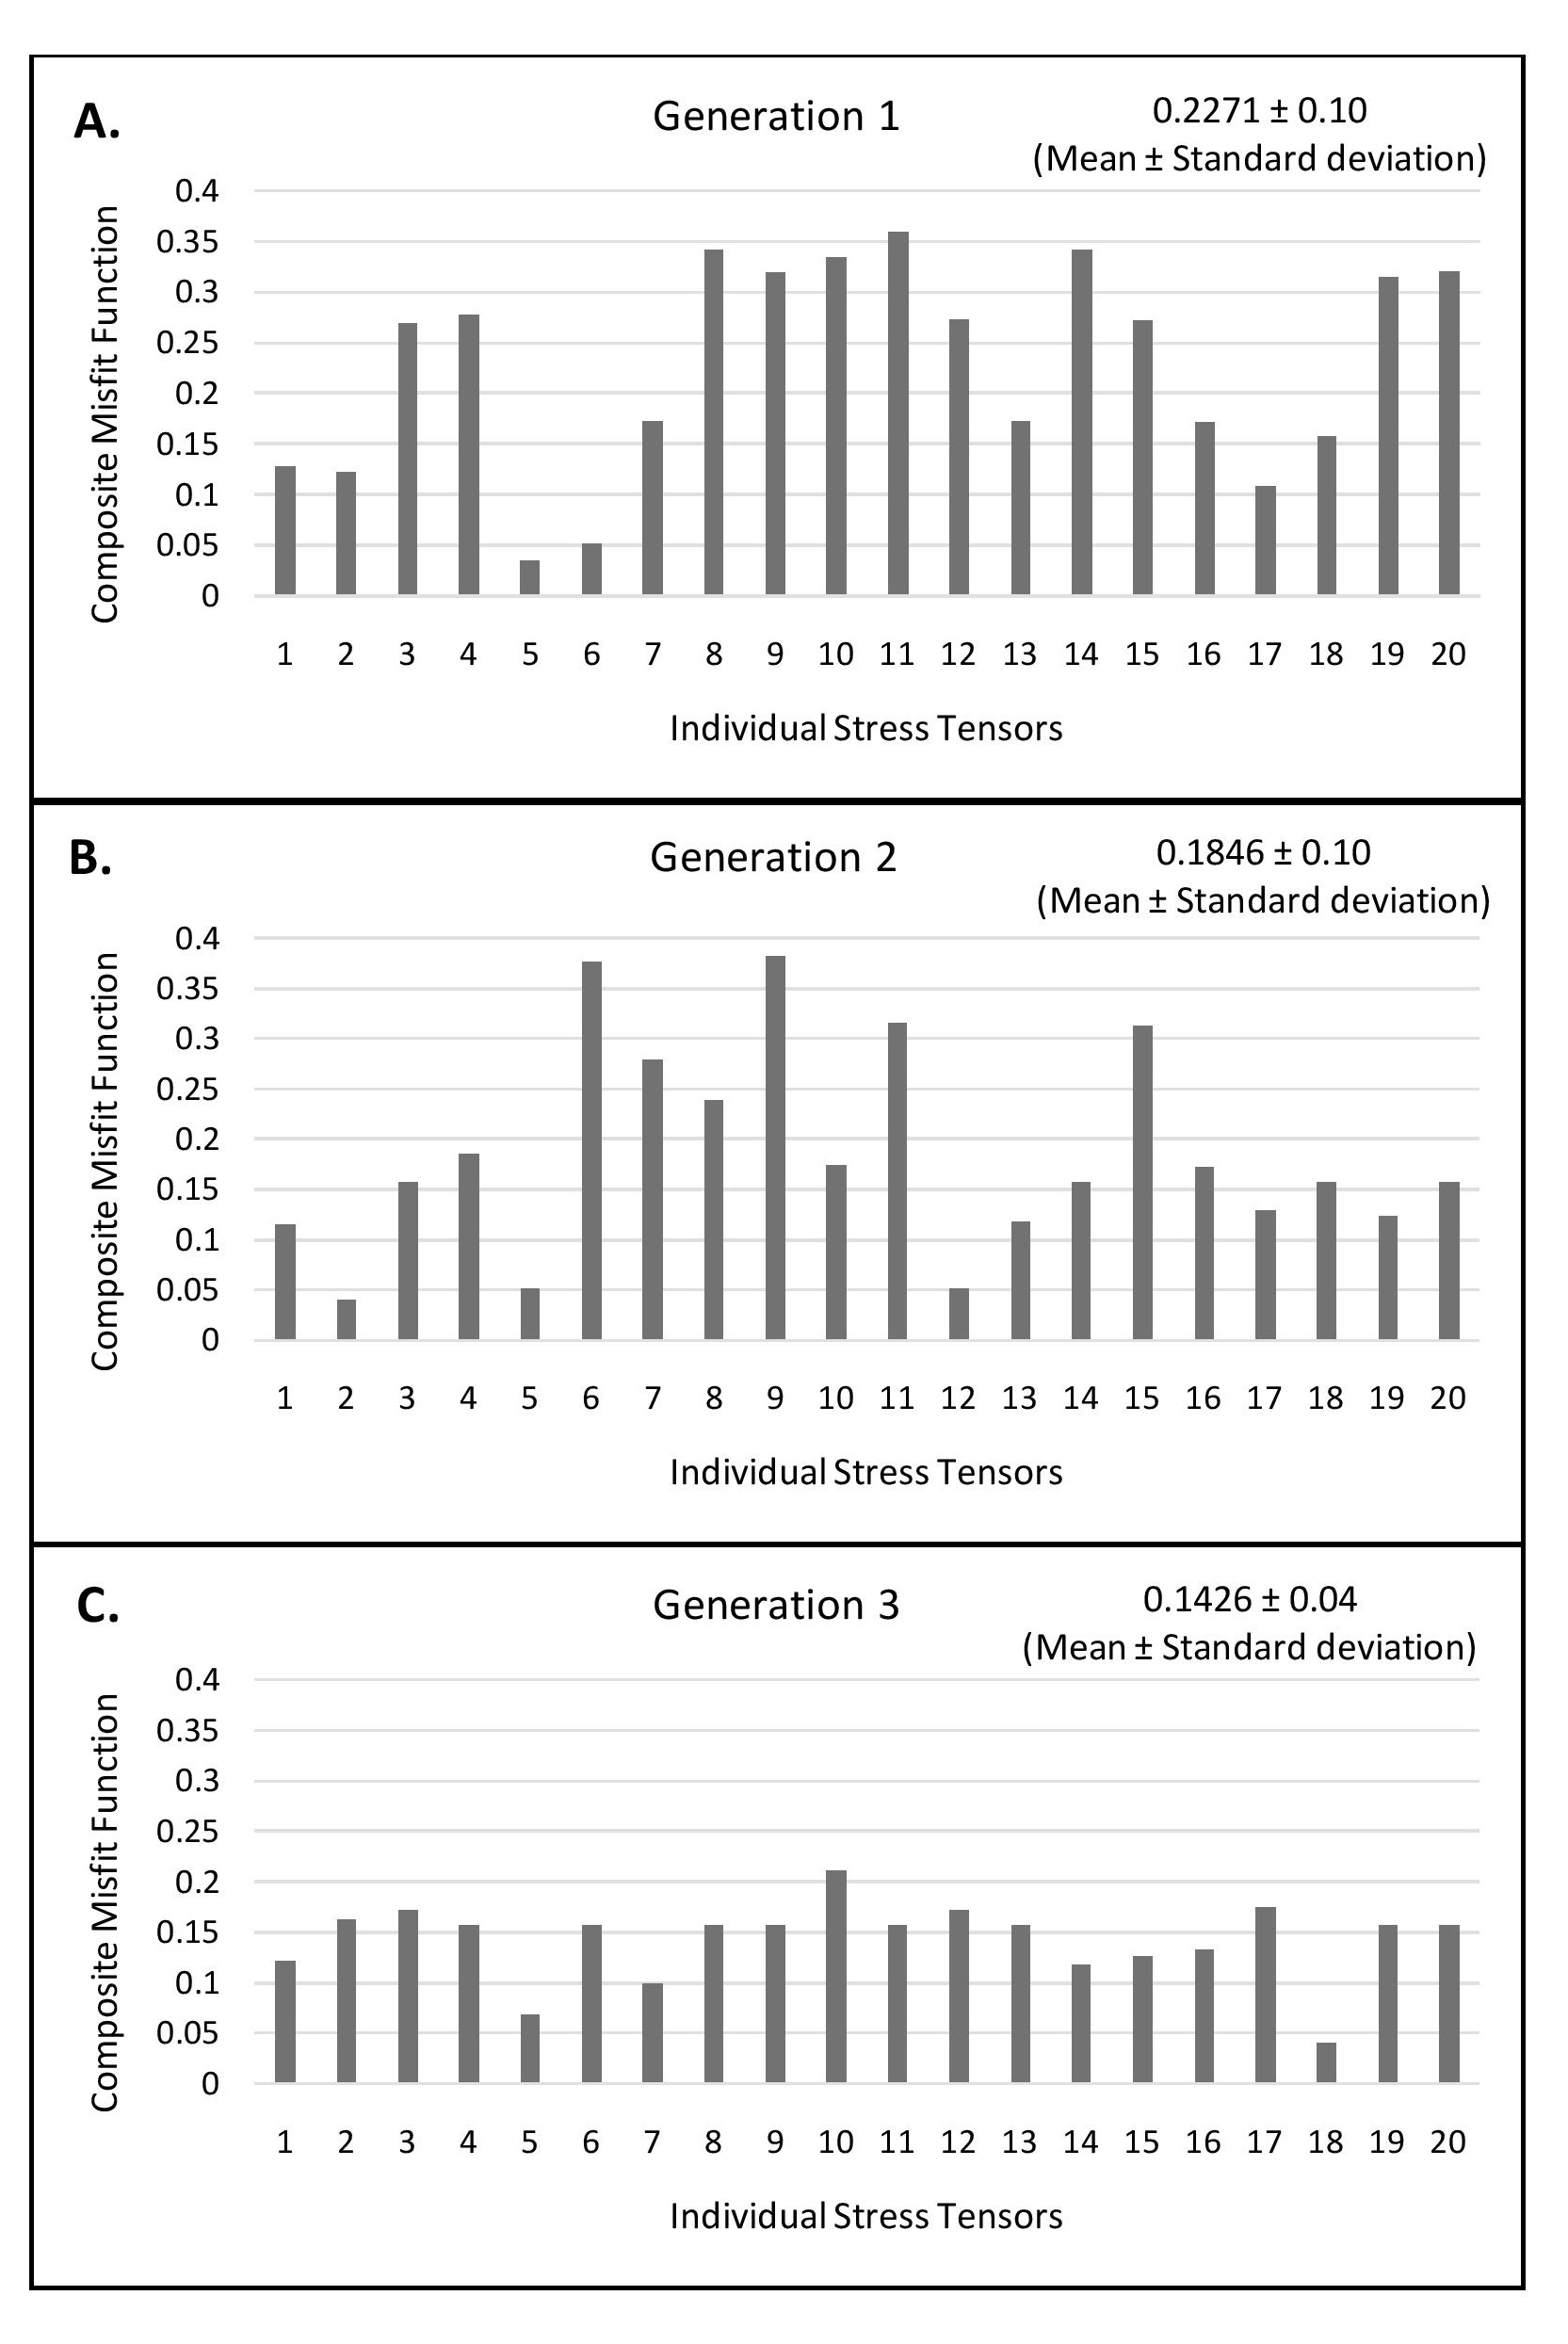
\includegraphics[scale = 1.0]{1}
\end{subfigure}
\end{figure}
\pagebreak
\begin{figure}[h!]
\ContinuedFloat
\begin{subfigure}{\textwidth}
    \centering
    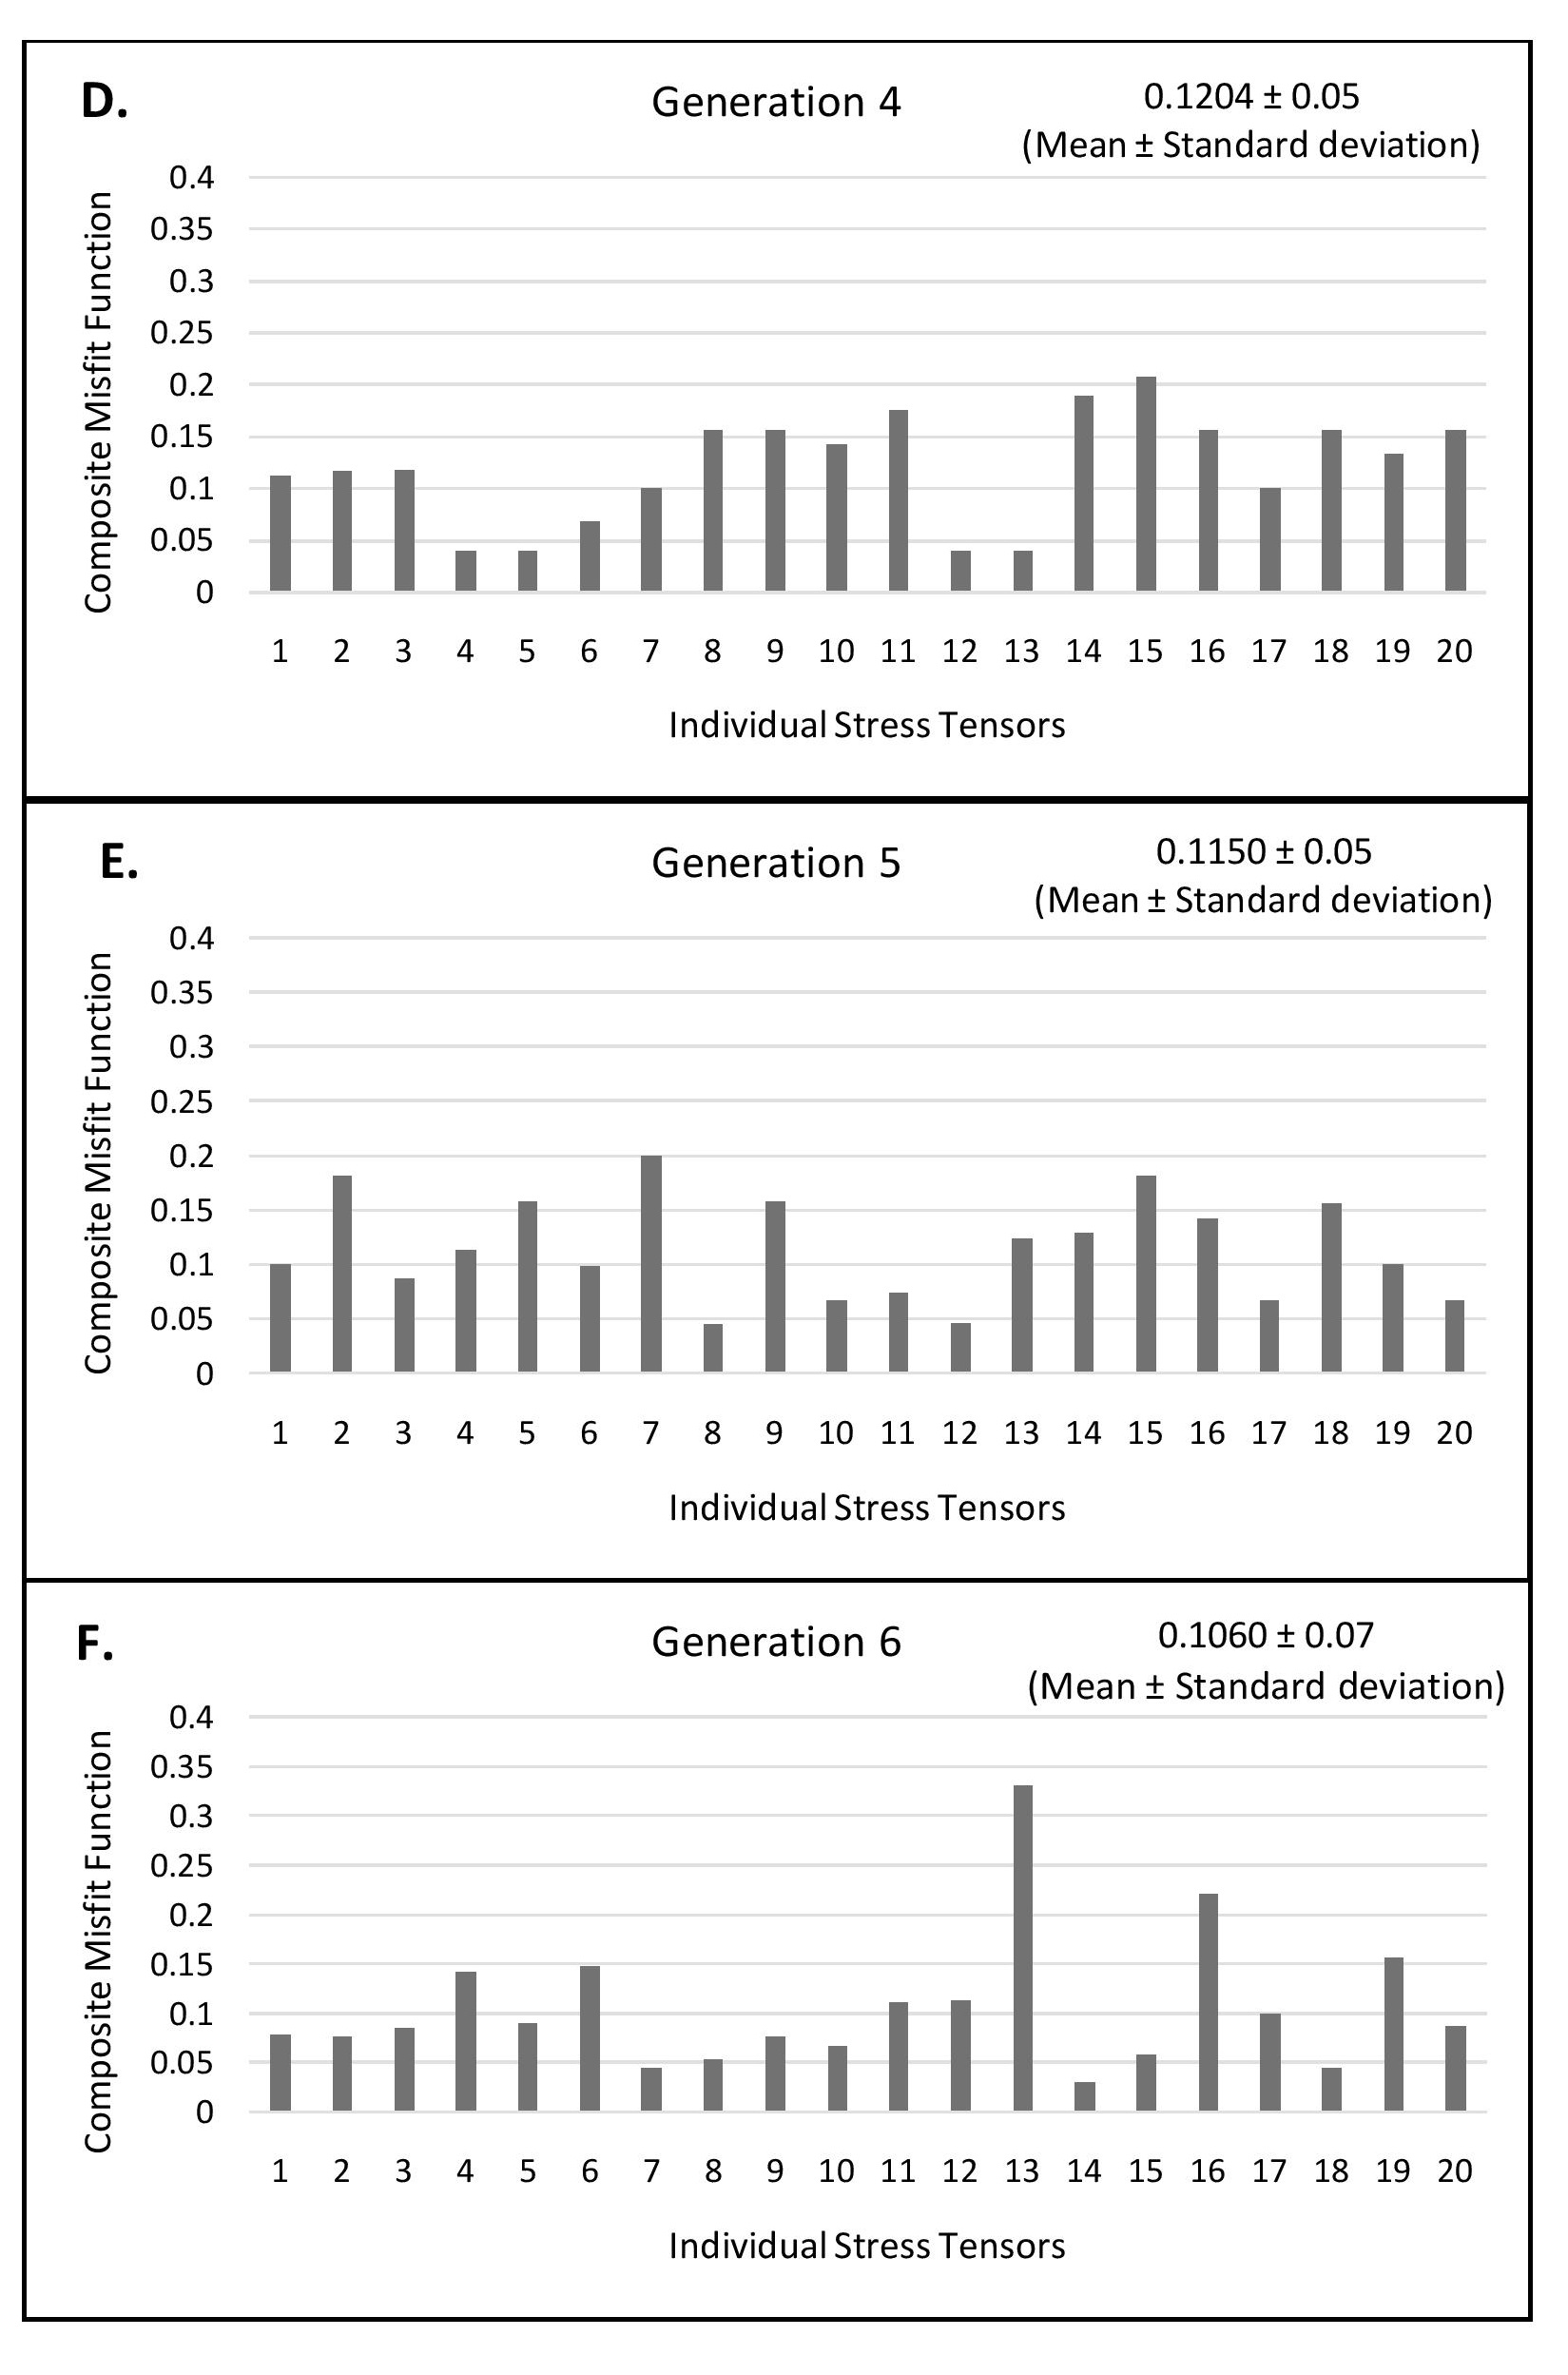
\includegraphics[scale = 1.0]{2}
\end{subfigure}
\end{figure}
\pagebreak
\begin{figure}[h!]
\ContinuedFloat
\begin{subfigure}{\textwidth}
    \centering
    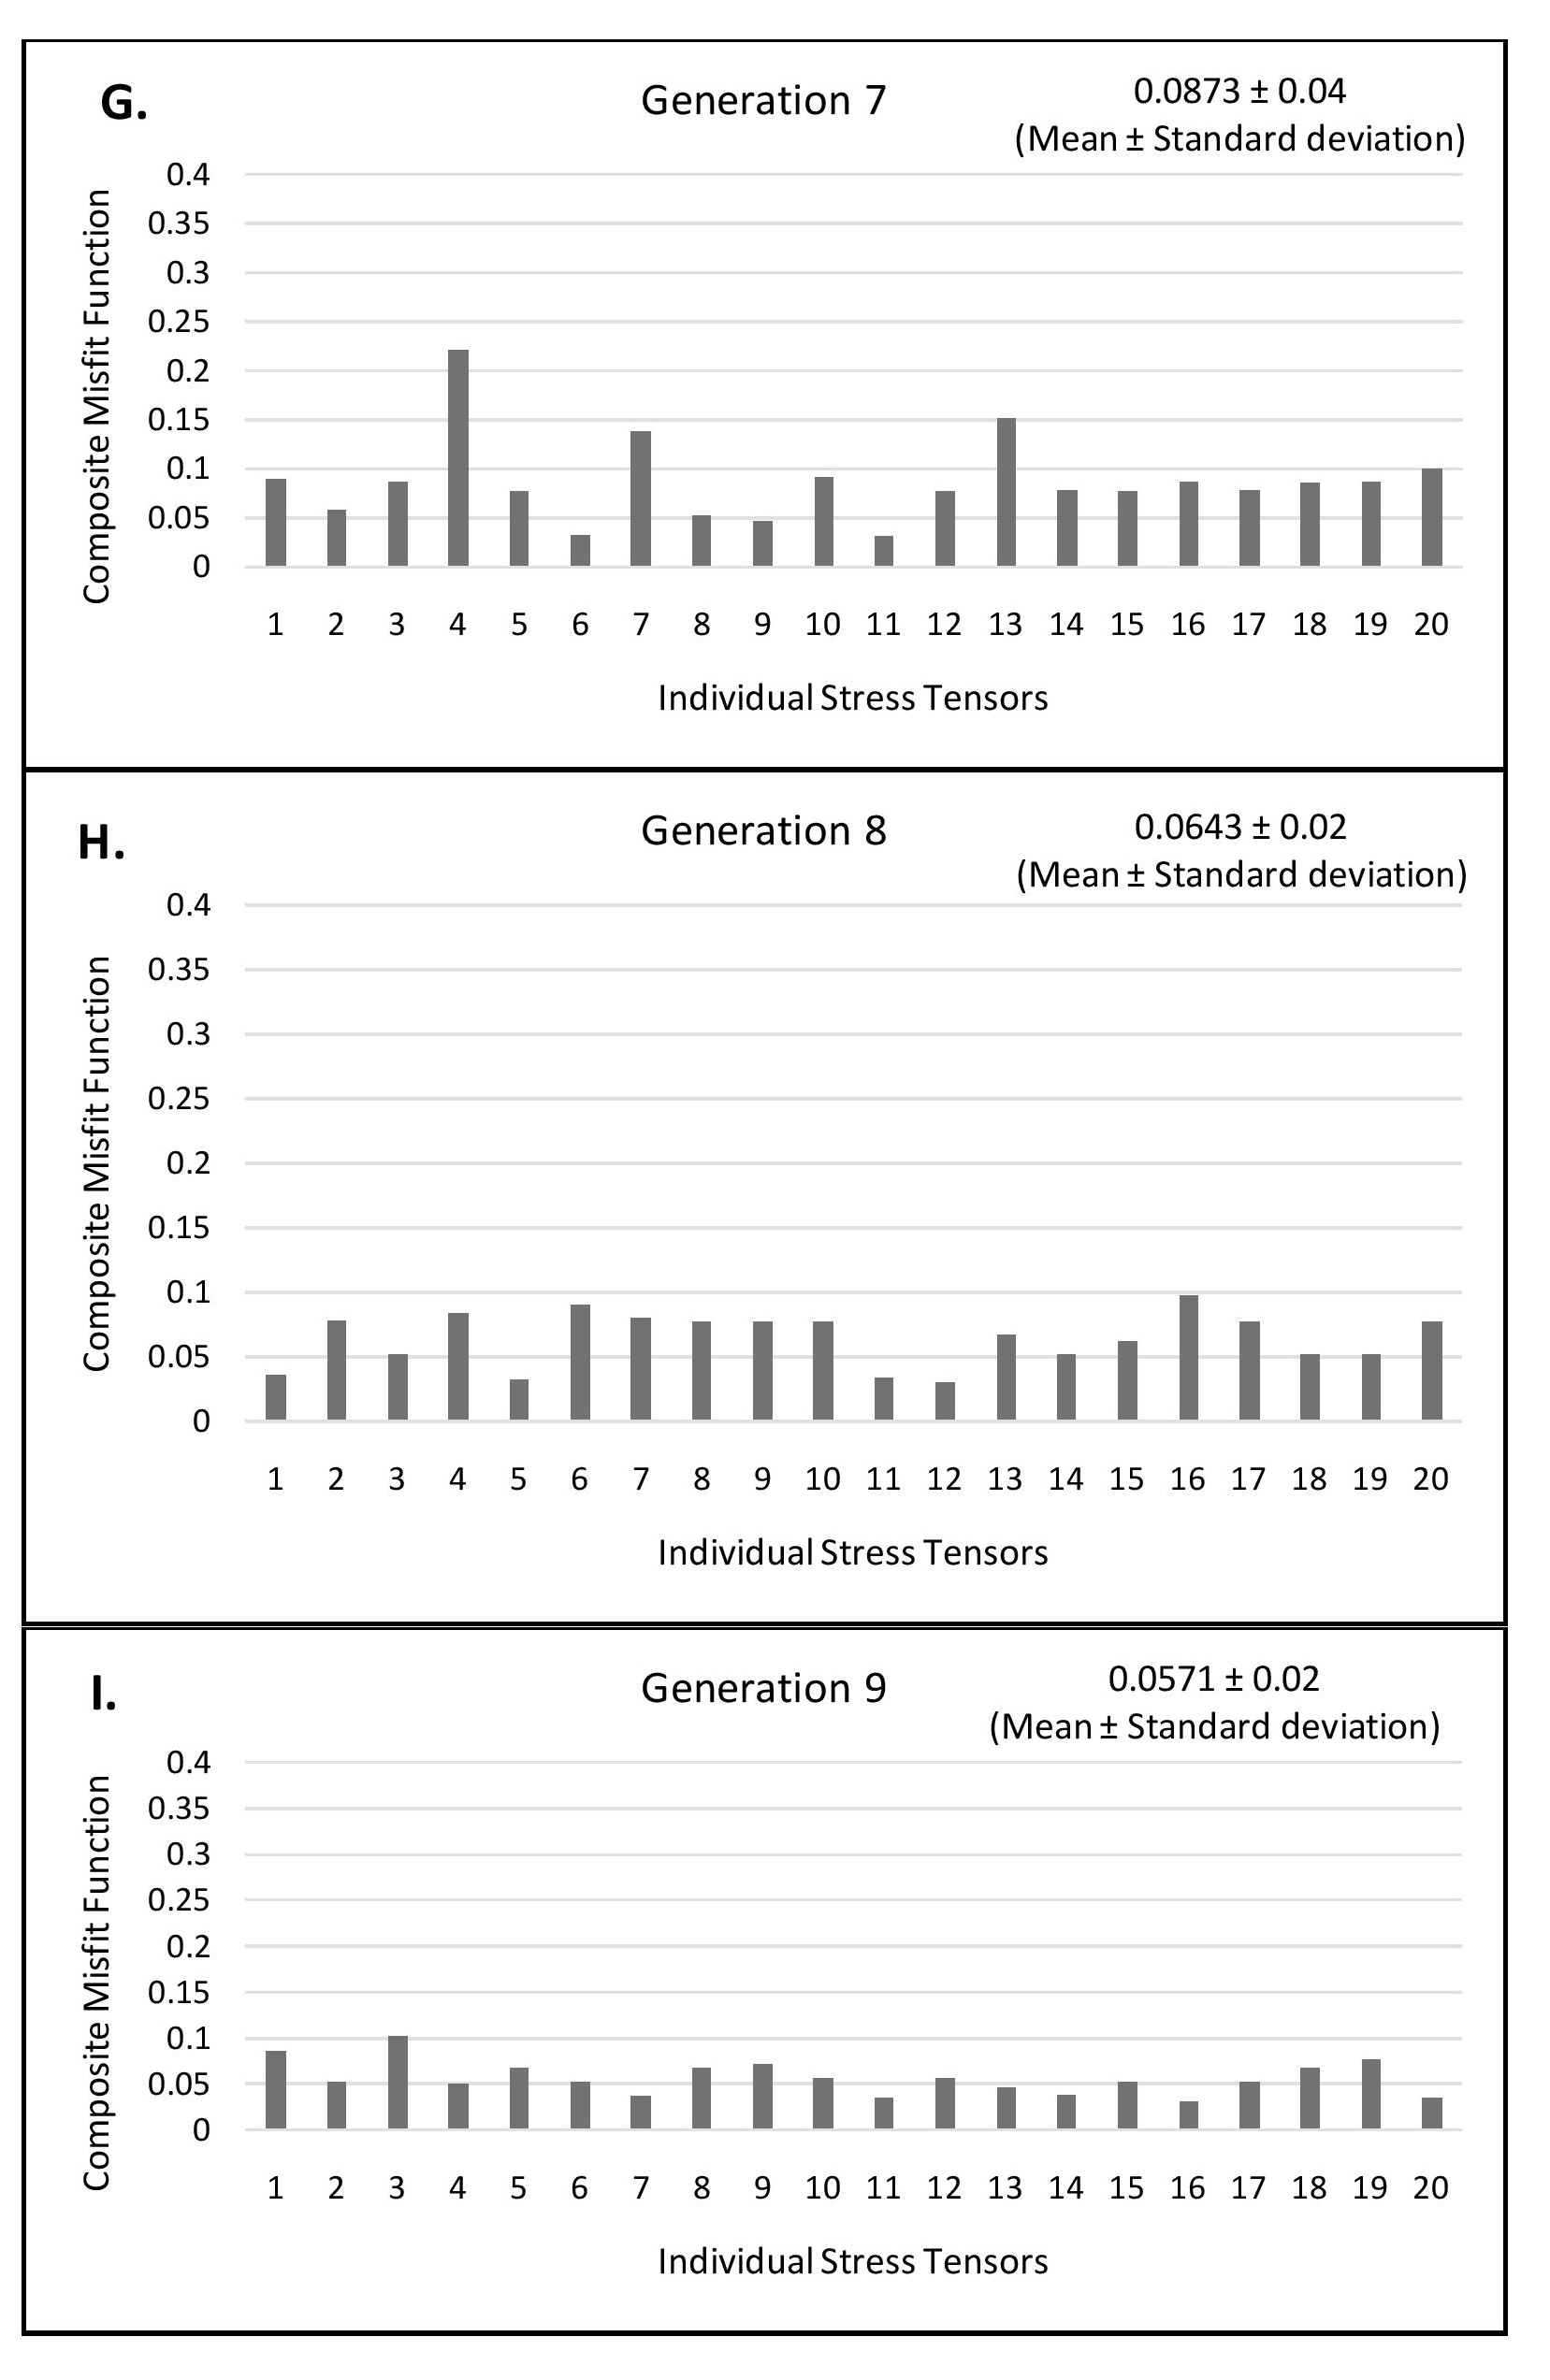
\includegraphics[scale = 1.0]{3}
\end{subfigure}
\end{figure}
\pagebreak
\begin{figure}[htb]
\ContinuedFloat
\begin{subfigure}{\textwidth}
    \centering
    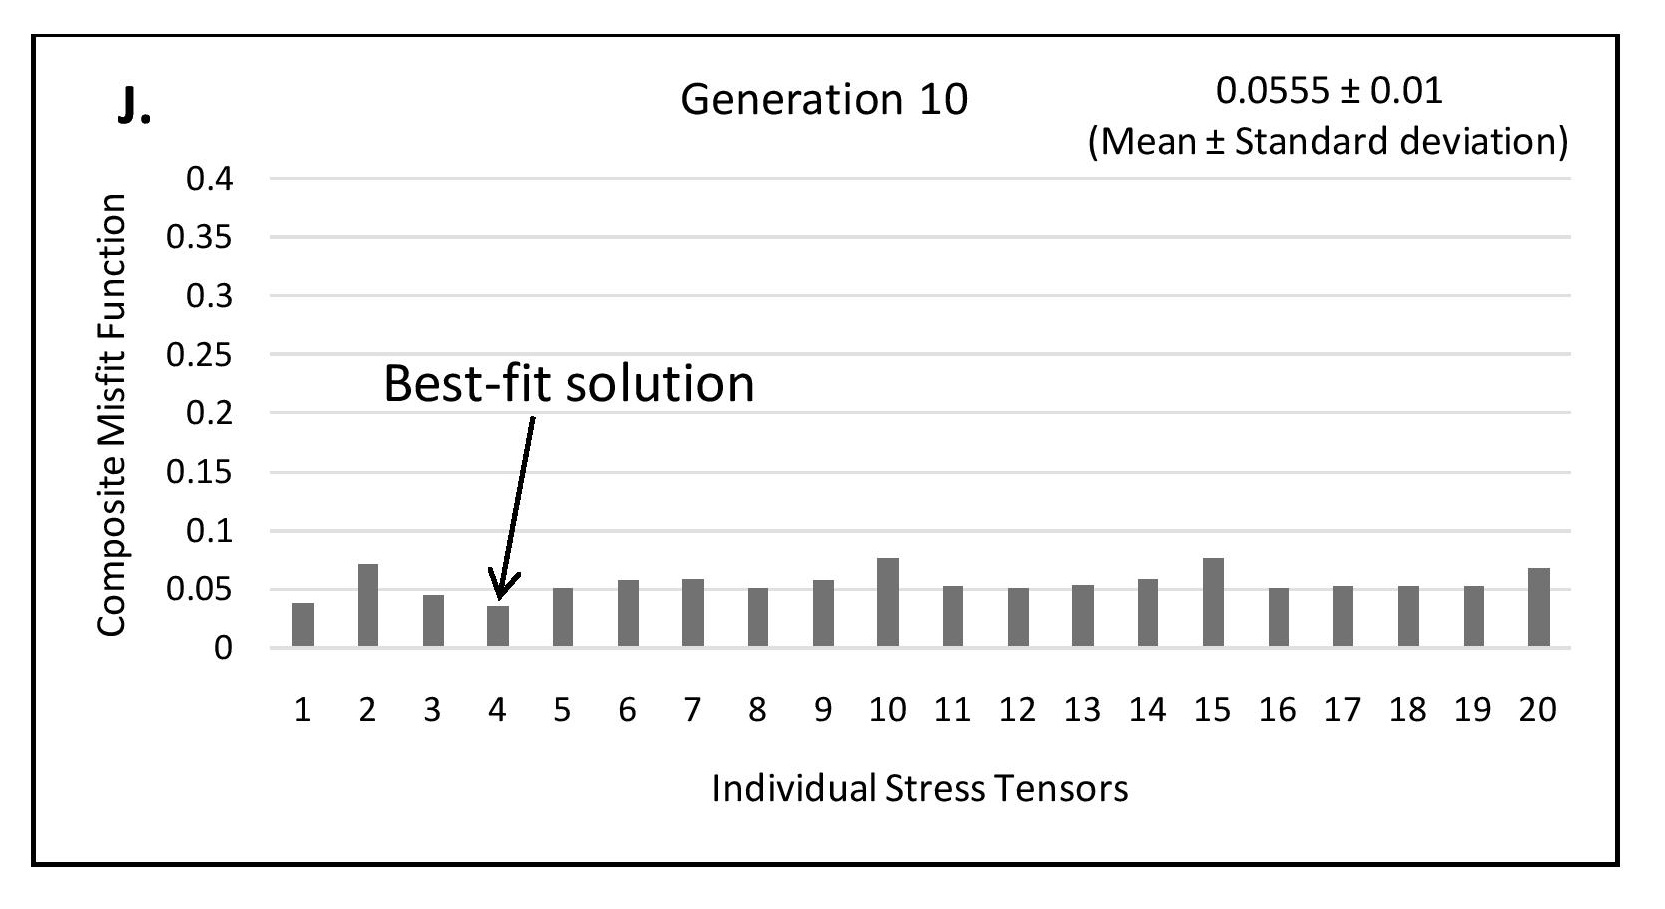
\includegraphics[scale = 1.0]{4}
\end{subfigure}
\caption{\textbf{A-J}: Composite misfit function for 10 iterations of the GA.}
\end{figure}


As the average misfit reduces, better individuals are produced in successive generations (Fig. 8:A-J). In the given population, the average misfit $\pm$ standard deviation reduce from $0.2271 \pm 0.10$ in the 1st generation to $0.0555 \pm 0.01$ in the 10th generation (Fig. 8:A-J). The 4th tensor in $10^{th}$ generation, having minimum composite misfit, is the optimum and required solution (Fig. 8:J).